\chapter{Implementacja}
\label{cha:implementacja}

W tym rozdziale opisana jest realizacja praktyczna projektu. Najpierw omówione zostaną wymagania stawiane całej aplikacji i omówione zostaną podstawowe
założenia związane z jej implementacją. Nastepnie przybliżone zostaną jej poszczególne komponenty.

\section{Wymogi i założenia}
\label{sec:wymogi}

\subsection{Budowa}
\label{subs:budowaAplikacji}

Podstawowym celem projektu jest implementacja oprogramowania pobierającego z podzbioru stron opublikowanych w Internecie dokumenty i przedstawiającego
je w postaci omówionych w Rozdziale \ref{cha:budowaGrafu} asocjacyjnych grafów AGDS. Jest to zadanie wieloetapowe, wymagające następujących komponentów:
\begin{enumerate}
\item Robota dostarczającego dane z sieci. Komponent musi mieć możliwość asynchronicznego pobierania stron WWW, udostępniać API do estrakcji adresów URL z ostatnio
ściągniętych stron spełniających podane warunki oraz implementować \emph{Robots Exclusion Protocol}.
\item Komponentu współpracującego z wyżej opisanym modułem, zapweniającego interfejs umożliwiający zapisywanie danych do zewnętrznej bazy. Umożliwiającego
zapisaywanie kolejnych wersji stron WWW, opisanych \emph{timestampem}.
\item Modułu przetwarzającego wybrane strony WWW przechowywane w zewnętrznej bazie. Powinien on być dawać możliwość parsowania strony HTML i operowania na drzewie DOM.
Powinien mieć możliwość zapisu informacji w formacie JSON, przy zachowaniu budowy umożliwiającej proste rozszerzanie funkcjonalności poprzez dodawanie odpowiednich klas do projektu.
\item Prostego klienta kolejki RabbitMQ, wykonującego RPC z przetworzonymi wcześniej danymi, jako argumentem.
\item Serwera odbierającego wywołania przez kolejkę RabbiMQ, rozpoczynającego konwersję danych do formatu AGDS i zwracającego wynik na kolejkę.
\item Modułu przetwarzającego dane odebrane przez serwer, dzielącego wysyłane strony na sekwencje uczące, umożliwiającego w razie potrzeby proste rozszerzenie funkcjonalności.
\item Silnika asocjacyjnego współpracującego z warstwą zapewniajacą persystencję. Jego jedynym zadaniem jest budowa grafu AGDS zgodnie z założeniami opisanymi w Rozdziale
\ref{cha:budowaGrafu}.
\item Warstwy pośredniczącej pomiędzy aplikacją, a bazami danych. Powinna ona zapisywać logiczną strukutrę grafu w bazie grafowej, a dodatkowe informacje, takie jak
atrybuty poszczególnych węzłów(np. częstość występowania), czy krawędzi(np. waga) przechowywać wlekkiej bazie klucz - wartość. Ważne jest ukreywanie szczegółów implementacyjnych,
zwłaszcza wynikających z używania wielu rodzajów baz danych.
\end{enumerate}

Zanim struktura aplikacji zostanie omówiona w większym detalu, należy opisać platformę, na której powstawała. W związku, z faktem, iż implementacja jest pewnego rodzaju eskperymentem, 
od którego nie wyamga się produkcyjnej sprawności, zaimplementowano ją w języku programowania Ruby. Pozwala on na szybką implementację nowych funkcjonalności, jest w pełni obiektowym i
bardzo elastycznym językiem programowania. Jednak związku z tym, iż Ruby jest językiem interpretowanym i posiada dynamiczne typowanie, zaawansowane możliwości metaprogramowania i 
zapewnia rozbudowane mechanizmy refleksji jego wydajność nie jest duża.
W związku z charakterystyką wybranej platformy program ma szanse działać poprawnie jedynie dla systemów typu Unix(Linux, OS X). Zstosowane zostały dwie wersje interepreterów Ruby'ego:
elementy 1. - 4. wymagają interpretera MRI, wersji conajmniej 2.0.0. Jest to pierwsza implementacja tego języka, napisana w C, większość najważniejszych gemów(bibliotek) jest dostępna 
przede wszystkim dla tej dystrybucji. Natomiast moduły 5. - 8. wymagają użycia alternatywnej implementacji na JVM, o nazwie JRuby. Jest to wymaganie używanej bazy grafowej i jest głównym 
powodem użycia kolejki RabbitMQ do komunikacji między dwoma głównymi częściami aplikacji.

Aplikacja używa 3 baz danych: PostgreSQLa(\url{http://www.postgresql.org/}) do przechowywania ściągniętych stron, Neo4j(\url{http://www.neo4j.org/}) jako bazy grafowej i Redisa(\url{http://redis.io/})
 jako lekkiej bazy klucz - wartość. Wszystkie posiadają biblioteki umożliwiające interakcje z nimi na poziomie obiektów języka, co znacznie ułatwia projektowanie aplikacji. Również każda
 z technologii używanych w projekcie jest technologią \emph{Open Source}.
 
 Każdy komponent posiada testy jednostkowe.

\begin{figure}[!h]
    \centering
    \label{graph:aplikacja}
    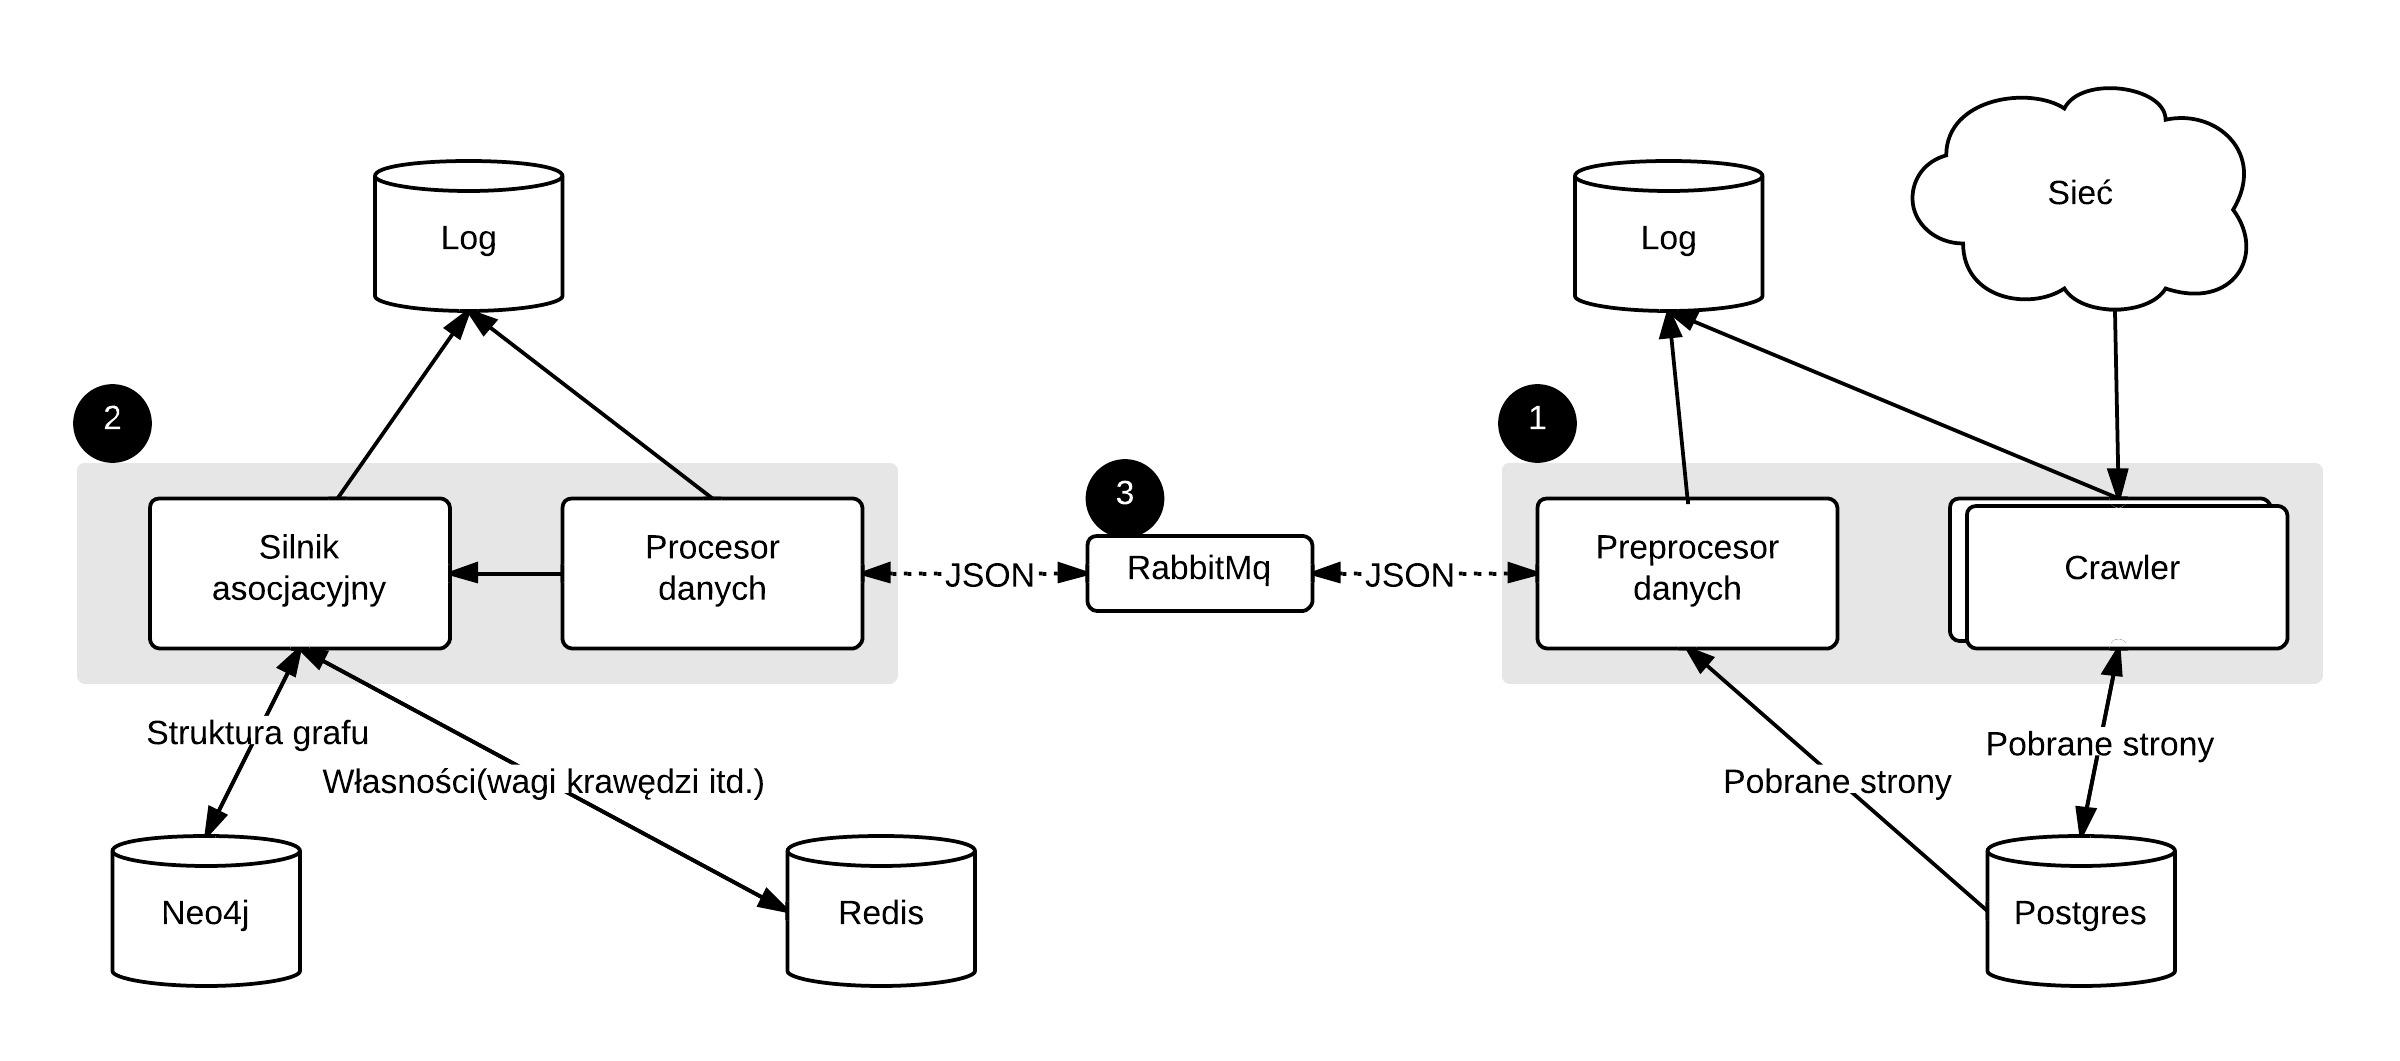
\includegraphics[scale=0.2]{aplikacja}
    \caption{Schemat architektury aplikacji. 1. - część napisana w MRI, 2. - część napisana w JRubym 3. - kolejka}
\end{figure}

\subsection{Wejście/wyjście}
\label{subsec:weWy}

Aplikacja nie posiada interfejsu graficznego. Poszczególne komponenty są wzbudzane z poziomu \emph{shella}, konfiguracja odbywa się poprzez edycję wydzielonych plików konfiguracyjnych, 
opcje podawane przy wykonywaniu skryptów lub zmienne środowiskowe. Celem tej części projektu nie jest serwowanie użytkownikowi informacji, a przedstawianie danych w pewny określonym
formacie, stąd takie ograniczone spektrum możliwości interakcji z aplikacją. Konkretne skrypty uruchamiające aplikacje, opcje ich wywoływania i struktura plików konfiguracyjnych opisana 
jest w dalszej części pracy.

\subsection{Wymagania instalacyjne}
\label{subs:wymaganiaInst}

Aplikacja byla rozwijana i testowana pod systemami typu Unix. Do instalacji i uruchomienia potrzebne są:
\begin{itemize}
\item system kontroli wersji Git (\url{http://git-scm.com/}),
\item Ruby zainstalowany za pomocą systemu kotroli wersji(preferowany rbenv - \url{http://rbenv.org/}),
\item Bundler (\url{http://bundler.io/}) i RubyGems (\url{http://rubygems.org/}),
\item serwer PostgreSQL,
\item baza grafowa Neo4j,
\item serwer Redis.
\end{itemize}

Instrukcje instalacji, konfiguracji i uruchamiania poszczególnych komponentów znajdują się w dalszych częściach pracy.

\section{Opis komponentów 1. - 4.}

Na rysunku \ref{graph:mri} przedstawiony jest detaliczny schemat pierwszych czterech komponentów głównej aplikacji. W istocie tworzą one autonomiczną subaplikację, powiązaną z resztą
komponentów jedynie poprzez kolejkę RabbitMQ. 

\begin{figure}[!h]
    \centering
    \label{graph:mri}
    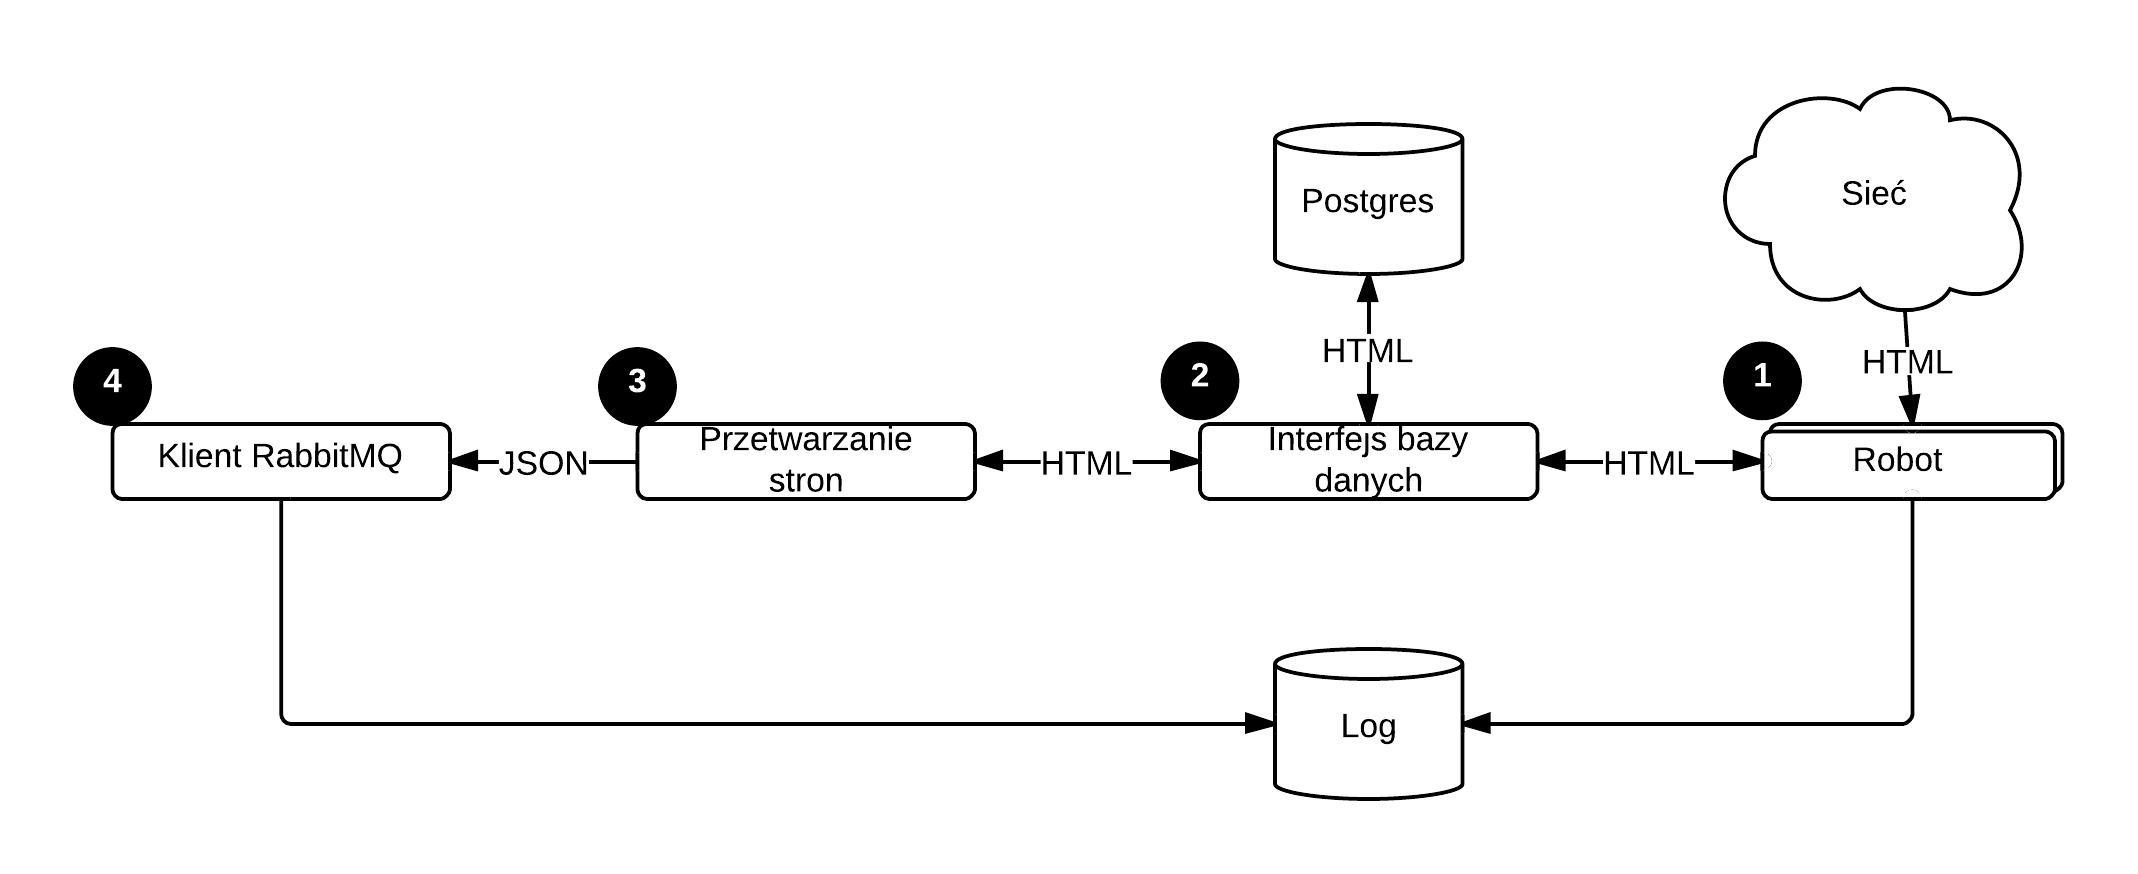
\includegraphics[scale=0.22]{mri}
    \caption{Detaliczny schemat komponentów 1. - 4. Podpisy na strzałkach odnoszą się do formatu, w jakim przedstawiane są strony internetowe na każdym z prezentowanych etapów. }
\end{figure}

\subsection{Konfiguracja}
\label{subs:konfiguracjaMri}

Konfiguracja możliwa jest poprzez dwa pliki znajdujące się w katalogu \texttt{./config}: \texttt{database.yml} i \texttt{config.yml}. Umożliwiają one dostarczenie potrzebnych
informacji pozwalających na połączenie z relacyjną bazą danych, jak i na konfigurację zachowania aplikacji. Poniżej przedstawiony jest listing obu plików 
wraz z wyjaśnieniem dostępnych opcji.

\texttt{database.yml}

\lstset{language=ruby}
\begin{lstlisting}[frame=single]
defaults: &defaults
  adapter: postgresql
  encoding: unicode
  pool: 5
  username: user
  password: pass
  host: localhost

development:
  database: taskmaster_dev
  <<: *defaults
test:
  database: taskmaster_test
  <<: *defaults

\end{lstlisting}

Jest to plik instrumentujący używany w aplikacji ORM - \emph{Active Record}, w celu umożliwienia połączenia z bazą. Konieczne podanie jest typu(\emph{adapter}), 
użytkownika(\emph{user}), hasła(\emph{password}) i lokazlizacji bazy(\emph{host}). Zdefiniowano również specjalne środowisko testowe, dostępne pod luczem \texttt{test}.
Służy ono do definicji bazy powoływanej do egzystencji na czas testów, a następnie bezpowrotnie niszczonej. 

\texttt{config.yml}

\lstset{language=ruby}
\begin{lstlisting}[frame=single]
crawler:
  connections: 20
  fetch_limit: 20
  url_pattern: '\/\/en\.wikipedia\.org\/wiki\/(?!\/|[A-Za-z]+:)'
  starting_page: 'http://en.wikipedia.org/wiki/Main_Page'
queue:
  limit: 50
logger:
  file: 'log/development.log'
  enabled: true

\end{lstlisting}

Plik ten przechowuje informacje konfiguracyjne aplikacji. Kolejno, odpowiadają one za:
\begin{itemize}
\item \texttt{crawler: connections} mówi, ile jednoczesnych asynchronicznych połączeń może wykonywać jeden proces robota.
\item \texttt{crawler: fetch\_limit} określa, ile na raz URLi jest wysyłanych do robota w celu ściągnięcia z Internetu. Nie jest t jednoznaczne z parametrem \texttt{connections}, 
w razie wysłania większej ilości adresów URL, niż jest otwieranych połączeń crawler wykona kilka iteracji i zwróci dokumenty odpowiadające wszystkim adresom.
\item \texttt{crawler: url\_pattern} przechowuje wyrażenie regularne, używane do filtracji adresów URL pobieranych ze stron. Jedynie adresy zgodne z wyrażeniem są zapamiętywane w bazie.
\item \texttt{crawler: starting\_page} podaje stronę startową, od której należy rozpocząć przeglądanie sieci.
\item \texttt{queue: limit} określa ile razy wywołana zostanie procedura przez kolejkę(ile stron zostanie wysłanych) przy jednym wywołaniu skryptu.
\item \texttt{logger: file} przechowuje relatywną wobec folderu projektu ścieżkę logowania.
\item \texttt{logger: enabled} to przełącznik, pozwalający na włąćzanie i wyłącznie loggera.
\end{itemize}

\subsection{Instalacja i uruchomienie}
\label{subs:instalacjaMri}

Po pobraniu repozytorum i upewnieniu się, że pliki konfiguracyjne zawierają odpowiednie wartości, należy za pomocą \emph{shella} wykonać następujące komendy:
\begin{enumerate}
\item \texttt{\$ bundle} - powoduje ściągnięcie wszystkich zależności,
\item \texttt{\$ rake db:create} - tworzy bazę,
\item \texttt{\$ PROJECT\_ENV=test rake db:create} -tworzy bazę testową,
\item \texttt{\$ rake db:migrate} - migruje bazę do scheme'y wymaganej przez aplikację.
\item \texttt{\$ PROJECT\_ENV=test rake db:migrate} - migruje bazę testową.
\item (opcjonalnie) \texttt{\$ rspec spec} w celu uruchomienia testów.
\end{enumerate}

Aby uruchomić robota internetowego należy w katalogu projektu wykonać polecenie
\texttt{\$ ./download}. W celu uruchomienia klienta kolejki RabbitMQ wystarczy w katalogu projektu wywołać \texttt{\$ ./publish}.
Aplikacja udostępnia również konsolę, umożliwiającą programiście interakcję z załadowanym środowiskiem. Aby z niej korzystać należy w katalogu projektu wywołać polecenie
\texttt{\$ ./console}. 
Zmienna środowiskowa \texttt{PRJOJECT\_ENV} używana jest do kontroli bazy danych, z którą łączy się aplikacja. Domyślnie przyjmuje ona wartość ``development'', a podczas testów
``test''. W celu uruchomienia np. konsoli z bazą testową, należy wywołać \texttt{\$ PROJECT\_ENV=test ./console}.

\subsection{Struktura przechowywanych informacji}
\label{subs:struktMri}

\begin{figure}[!h]
    \centering
    \label{graph:mri_schema}
    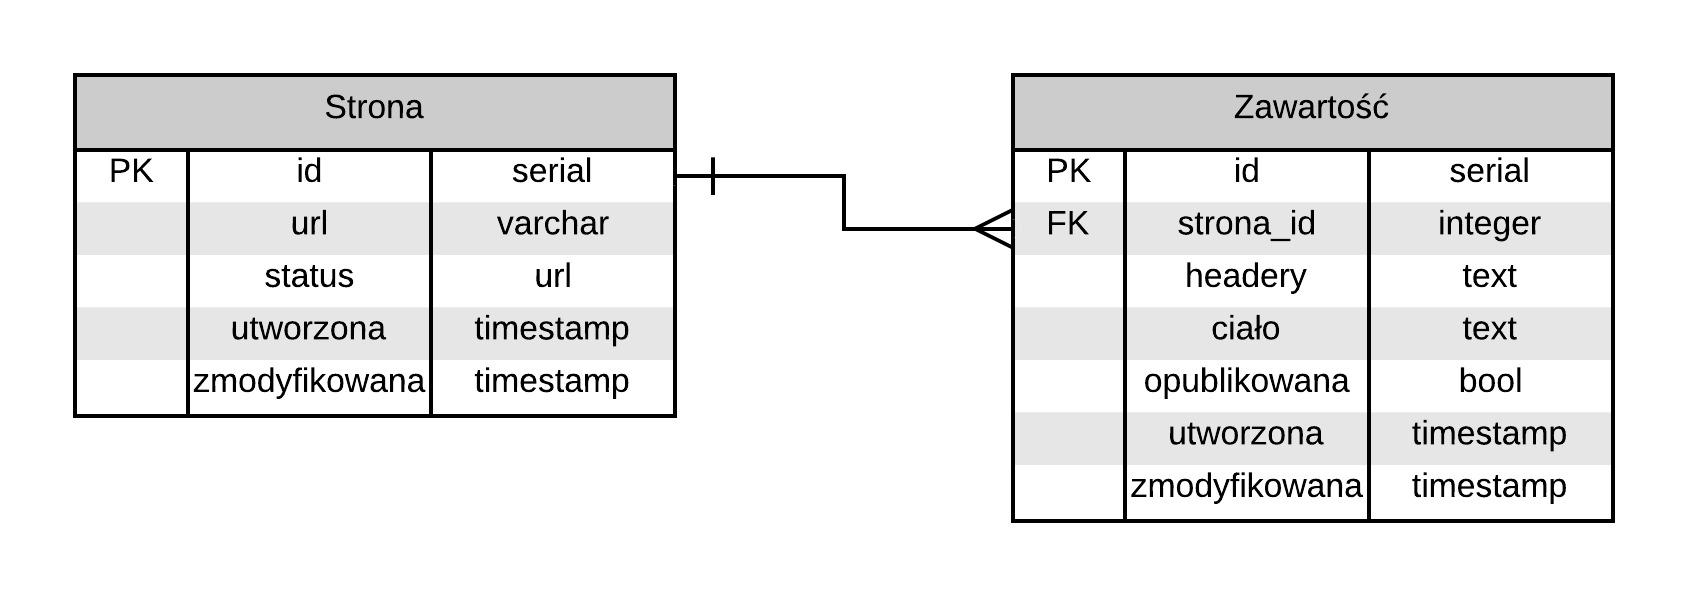
\includegraphics[width=\textwidth]{mri_schema}
    \caption{Schema przechowująca informacje pobrane z sieci.}
\end{figure}

Struktura bazy umożliwia przechowywanie unikalnych adresów URL w relacji \emph{Strona} i zapisywanie historii kolejnych odwiedzin w osobnej tabeli \emph{Zawartość}. Dzięki
temu otrzymuje się prosty sposób na archiwizację nieaktualnych rekordów, przy braku konieczności modyfikacji bazy. Następnie takie rekordy mogłyby być cyklicznie przenoszone 
np.~do hurtowni danych, w celu późniejszej analizy. Dodatkowego wyjaśnienia wymagają dwa pola: pole \texttt{strona.status} przyjmujące wartości ze zbioru: 
${oczekuje, pobierana, sukces, błąd}$, odpowiadające cyklowi pobierania i przetwarzania informacji. Wartość $pobierana$ ma na celu niedopuszczenie do pobierania tej samej
strony przez dwa procesy robota. Drugie to pole \texttt{wartość.opublikowana} odnosi się do faktu wysłania danej zawartości do kolejki. Jeżeli to nastąpiło i komponent nie otrzymał
w odpowiedzi zwrotnej komunikatu o błedzie, wartością tegopola będzie TRUE, w przeciwnym razie FALSE.

\subsection{Przepływ danych}
\label{subs:przepDanych}

Aplikacja posiada dwie niezależne ścieżki przepływu i przetwarzania danych:
\begin{enumerate}
\item Ścieżka związana z pobieraniem danych z sieci.
\item Ścieżka przetwarzania ściągniętych danych i publikacja ich za pomocą kolejki.
\end{enumerate}

Pierwsza ścieżka jest realizowana przez skrypt \texttt{download} i przedstawiona na rysunku \ref{graph:mri_przeplyw_1}. Uruchamia on robota, który po odczytaniu konfiguracji i nawiązaniu połączenia z bazą danych zaczyna pobierać
automatycznie dane z sieci.  Liczba procesów wykonujących to zadanie nie ma narzuconego z góry ograniczenia, dane między procesami są synchronizowane na poziomie dostępu do bazy danych.
Jak można zauważyć przedstawiony schemat nie różni się od podstawowej implementacji crawlera przedstaionej w rozdziale \ref{cha:pozyskiwanieTresci}.


Rolę listy adresów URL przejęła baza danych. Jest to może rozwiązanie nieefektywne, ale proste w implementacji i wystarczające dla niniejszego projektu.
W razie konieczności przyspieszenia działania robota można zastosować lekką bazę NoSQL, jak Redis, czy rozwiązanie cache'ujące, takie jak Memcached.
W celu oszczędzenia czasu, nie zawsze następuje ekstrakcja adresów URL i dodawanie ich do bazy. Nastepuje to jedynie wtedy, gdy liczba adresów oczekujących
jest mniejsza, niż czterokrotność liczby adresów odwiedzonych. 

Druga ścieżka przepływu danych ma prostszy przebieg, dlatego ograniczone się jedynie do wypisania jej poszczególnych kroków.
\begin{enumerate}
\item Pobranie nieopublikowanego(flaga \texttt{opublikowana} ma wartość FALSE) rekordu z tabel \texttt{Zawartość}.
\item Parsowanie ciała strony za pomocą biblioteki Nokogiri.
\item Pobranie z drzewa DOM interesujących elementów, np. całej zawartości umieszczonej między znacznikami HTML <p>\dots</p> i podzielenie jej na dwie grupy: pierwszą, która
obowiązkowo musi zostać użyta do budowy grafu AGDS(np. tekst umieszczony w nagłówkachi) i drugą, która zawiera przydatne, ale mniej wartościowe informacjue - np. tekst z ciała artyułu.
\item Podział tak przygotowanego tekstu na zdania i zapis do dwóch tablic, kolejno dla pierwszej i drugiej grupy.
\item Dodanie informacji o adresie URL przetwarzanej strony, zakodowanie jako JSON i opublikowanie poprzez kolejkę.
\end{enumerate}


\newpage

\begin{figure}[!h]
    \centering
    \label{graph:mri_przeplyw_1}
    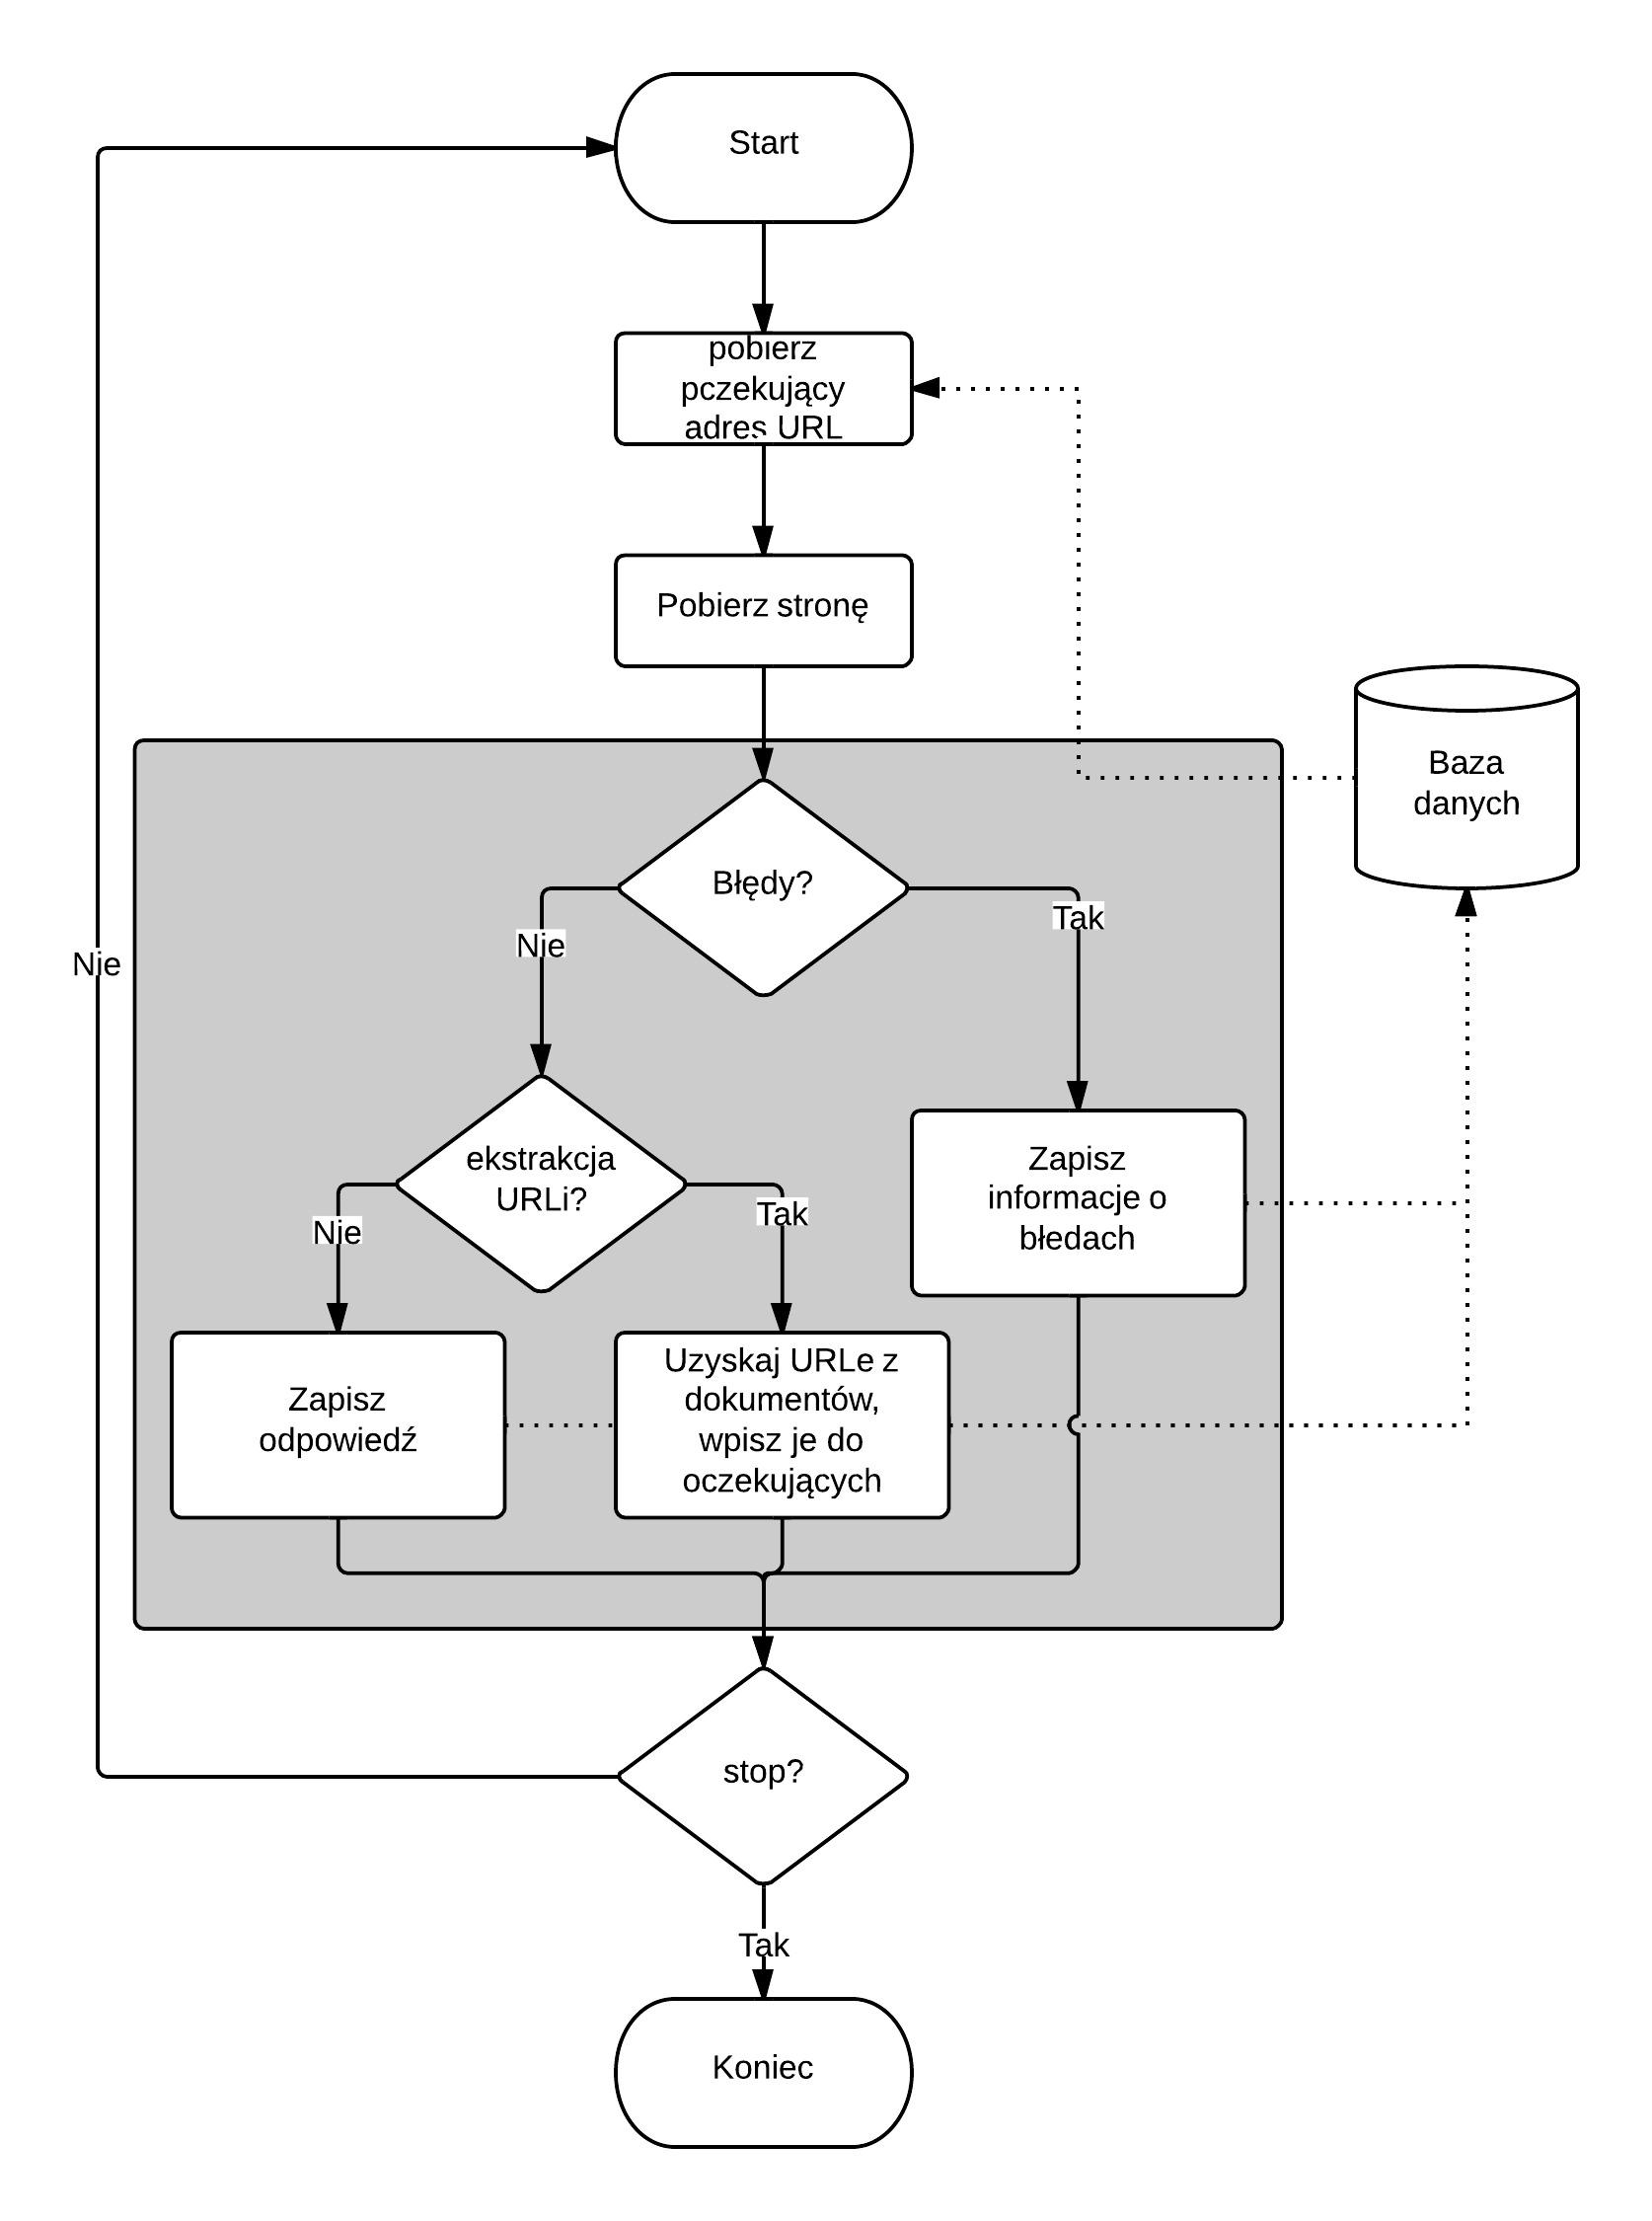
\includegraphics[width=\textwidth]{mri_przeplyw_1}
    \caption{Schemat pierwszej ścieżki przepływu. Dla przejrzystości nie uwzględniono asynchronicznego sposobu pobierania stron.}
\end{figure}



\section{Opis komponentów 5. - 8.}

Na rysunku \ref{graph:neo4j} przedstawiony jest detaliczny schemat reszty aplikacji. Jest to również kod pracujący autonomicznie, jedynym punktem wejścia
jest serwer nasłuchjący na kolejce RabbitMQ.

\begin{figure}[!h]
    \centering
    \label{graph:neo4j}
    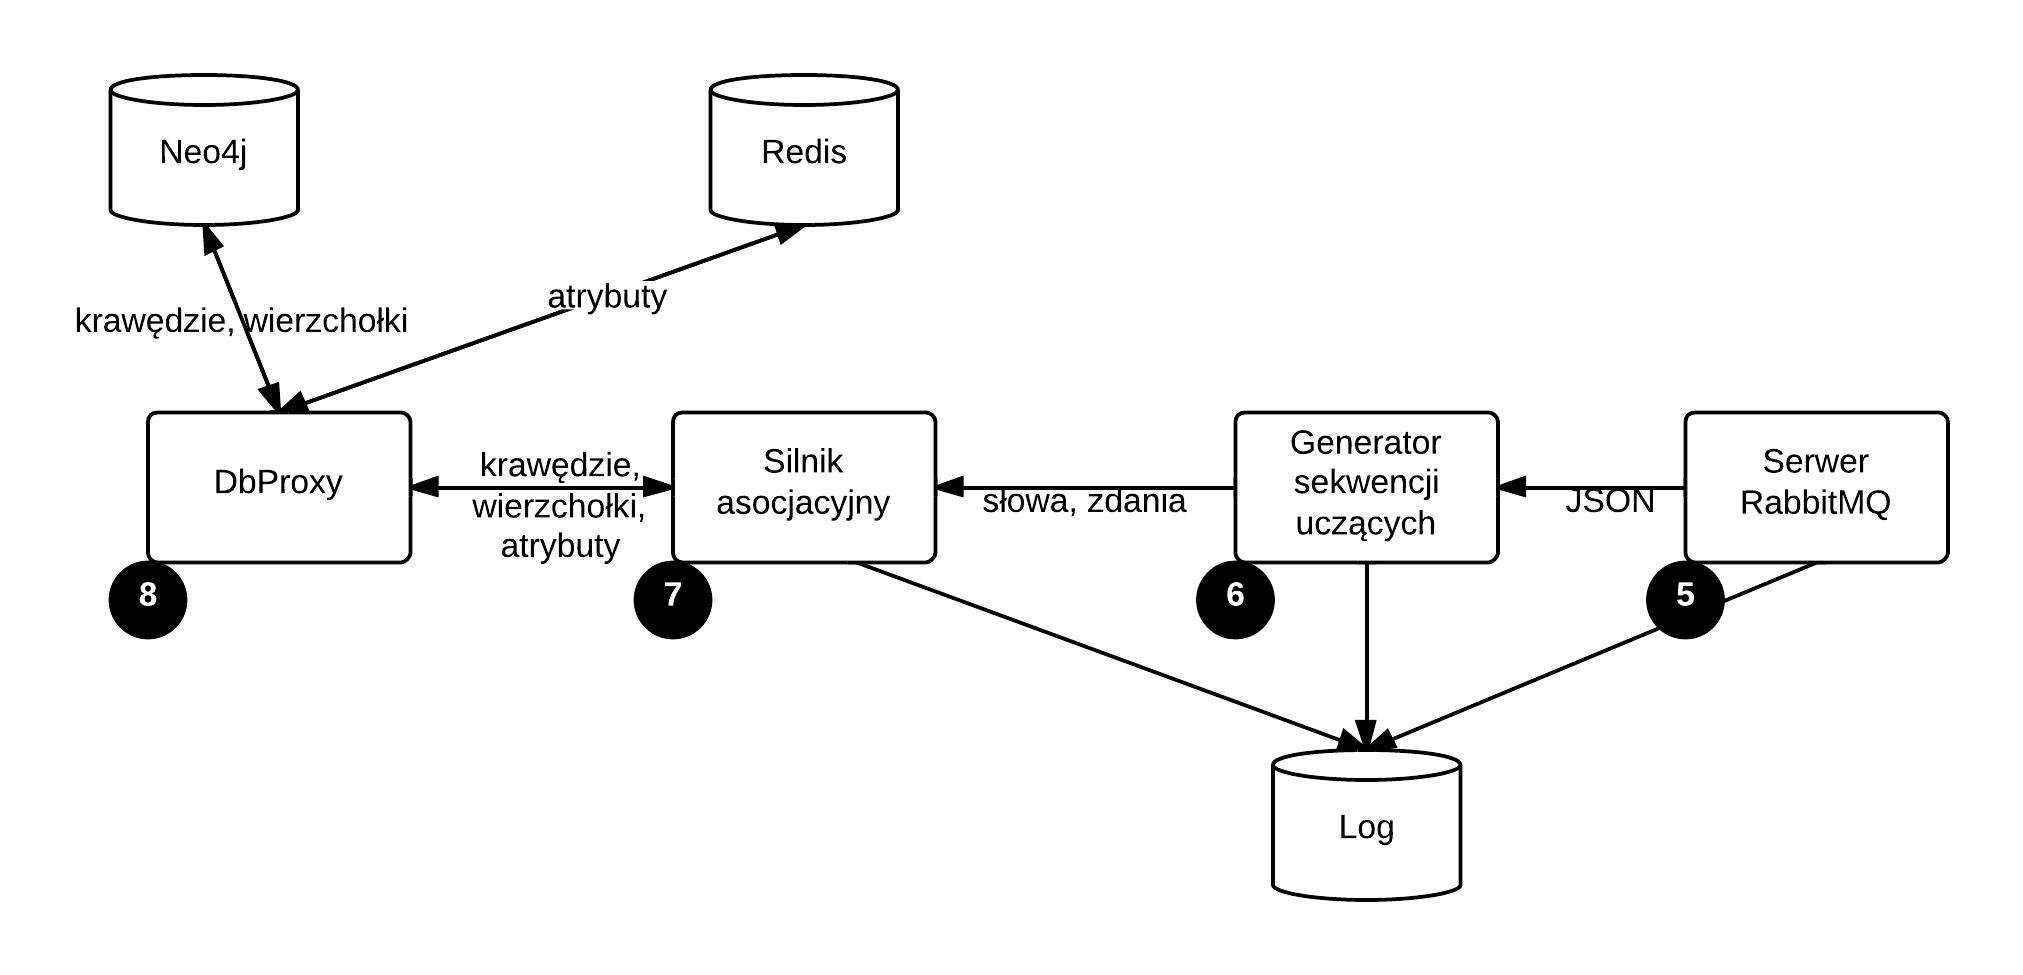
\includegraphics[scale=0.22]{neo4j}
    \caption{Detaliczny schemat komponentów 5. - 8. Podpisy na strzałkach odnoszą się do formy, jaką przyjmują przepływające przez aplikację dane.}
\end{figure}

\subsection{Konfiguracja}
\label{subs:konfiguracjaNeo4j}

Podobnie, jak opisana w sekcji \ref{subs:konfiguracjaMri} część projekt, również komponenty 5. - 8. są konfigurowane za pomocą pliku znajudującego się w katalogu 
\texttt{./config}: \texttt{config.yml}. Odpowiada on za przechowywanie informacji potrzebnych do połaczenia z bazami, lokalizacji plików z logami itd., jak i do 
ustalania parametrów silnika asocjacyjnego. Część opcji dotyczy również silnika symulacyjnego umożliwiającego przeprowadzanie eksperymentów z sieciami ANAKG, jednak
nie jest on bliżej omówiony w niniejszej pracy.

\lstset{language=ruby}
\begin{lstlisting}[frame=single]
payload:
  optional_limit: 2000
  min_word_length: 2
  max_word_length: 25
  max_sentence_length: 4

logger:
  enabled: true
  file: 'log/neo4ruby.log'

redis:
  host: '127.0.0.1'
  port: 6379

search_engine:
  simulation:
    alpha: 0.7
    beta: 0.8
    theta: 1.0
    initial_exc: 0.95
    max_iterations: 10
    min_change_rate: 0.2

  response_scanning:
    limit: 5
    levenshtein_max: 3
    # stopwords after http://www.webconfs.com/stop-words.php
    stopwords_file: 'data/stopwords'

  answer_resolving:
    limit: 10

experiment: 'exp1'

\end{lstlisting}
Poszczególne opcje odpowiadają za:
\begin{itemize}
\item \texttt{payload: optional\_limit} -  maksymalna ilość słów, która jest wprowadzana do bazy grafowej z pojedynczej sekwencji uczącej(pojedynczej strony).
\item \texttt{payload: min\_word\_length} - minimalna długość słowa(słowa krótsze są usuwane z sekwencji uczącej).
\item \texttt{payload: max\_word\_length} - maksymalna długość słowa, j.w.
\item \texttt{payload: max\_sentence\_length} - maksymalna długość zdania. Zdanie w aplikacji jest równoważne kontekstowi opisywanemu w rozdziale \ref{cha:budowaGrafu}.
\item \texttt{logger: enabled} - wł./wył. logowanie.
\item \texttt{logger: file} - lokalizacja pliku z logami.
\item \texttt{redis: } - dane potrzebne do połączenia z Redisem.
\item \texttt{search\_engine: } - parametry symulacji i asocjacyjnej wyszukiwarki internetowej.
\item \texttt{experiment: } - nazwa eksperymentu. Jest to \emph{de facto} ścieżka, w której przechowywane są pliki wbudowanej bazy grafowej. Zmieniając ją, zmienia się
bazę, z którą łączy się aplikacja.
\end{itemize}

\subsection{Instalacja i uruchomienie}
\label{subs:instalacjaMri}

Po pobraniu repozytorum i upewnieniu się, że pliki konfiguracyjne zawierają odpowiednie wartości, należy za pomocą \emph{shella} wykonać następujące komendy:
\begin{enumerate}
\item \texttt{\$ bundle} - powoduje ściągnięcie wszystkich zależności,
\item (opcjonalnie) \texttt{\$ rake test} w celu uruchomienia testów.
\end{enumerate}

Aby uruchomić serwer należy będąc w katalogu aplikacji wywołać polecenie \texttt{\$ ./start}. Przyjumje ono dwa opcjonalne argumenty: \texttt{-e -\--experiment EXP\_NAME} daje możliwość
ręcznego ustawienia bazy, z którą łączy się aplikacja. Zmienna ustawiona w ten sposób nadpisze konfigurację zapisaną w pliku; \texttt{-q -\--queue QUEUE\_NAME} pozwala na zmianę nazwy
kolejki, na której nasłuchuje serwer. Należy jednak wspomnieć, iż ustawienia te były wykorzystywane głównie do rozwoju aplikacji na jej wczesnym stadium, docelowo wszystkie ustawienia
zostaną przeniesione do pliku konfiguracyjnego.

Aplikacja posiada również skrypt ładujący całe środowisko i pozwalający na interaktywną jego eksplorację za pomocą linii komand. Uruchamiany jest on poleceniem \texttt{./console} z
folderu projektu. W razie, gdy istnieje potrzeba połączenia się z inną bazą, niż wyszczególniona w pliku konfiguracyjnym, można użyć opcji \texttt{-e -\--experiment EXP\_NAME}.

\subsection{Struktura przechowywanych informacji}
\label{subs:struktNeo4j}

Jak wspomniano wcześniej, baza grafowa cechuje się większą elastycznością, niż tradycyjne bazy relacyjne. Nie używa ona schematów, użytkownicy mają dowolność w kształtowaniu 
grafu i wielopoziomowych relacji łączących jego elementy. Z powodów wydajnościowych zdecydowano się na użycie dwóch rodzajów baz: Neo4j odpowiada za przechowywanie struktury grafu,
jego trawersowanie i integralność. To rozwiązanie stosowane jest ze względu na przyjazne API i łatwość integracji z aplikacją. Jednak ze wzgledu na duża ilość wpisów do bazy
podczas tworzenia struktury grafu AGDS(docelowo setki tysięcy stron) oraz konieczność sekwencyjnego budowania grafu, atrybuty elementów grafu, takie jak np. słowa wchodzące
w skład sekwencji uczącej, czy wagi krawędzi sa przechowywane przez prawie cały czas w pamięci programu i zapisywane okresowo w Redisie. Dzięki temu ograniczono znacząco ilość
kosztownych operacji I/O.

\begin{figure}[h!]
    \label{graph:logic_graph}
    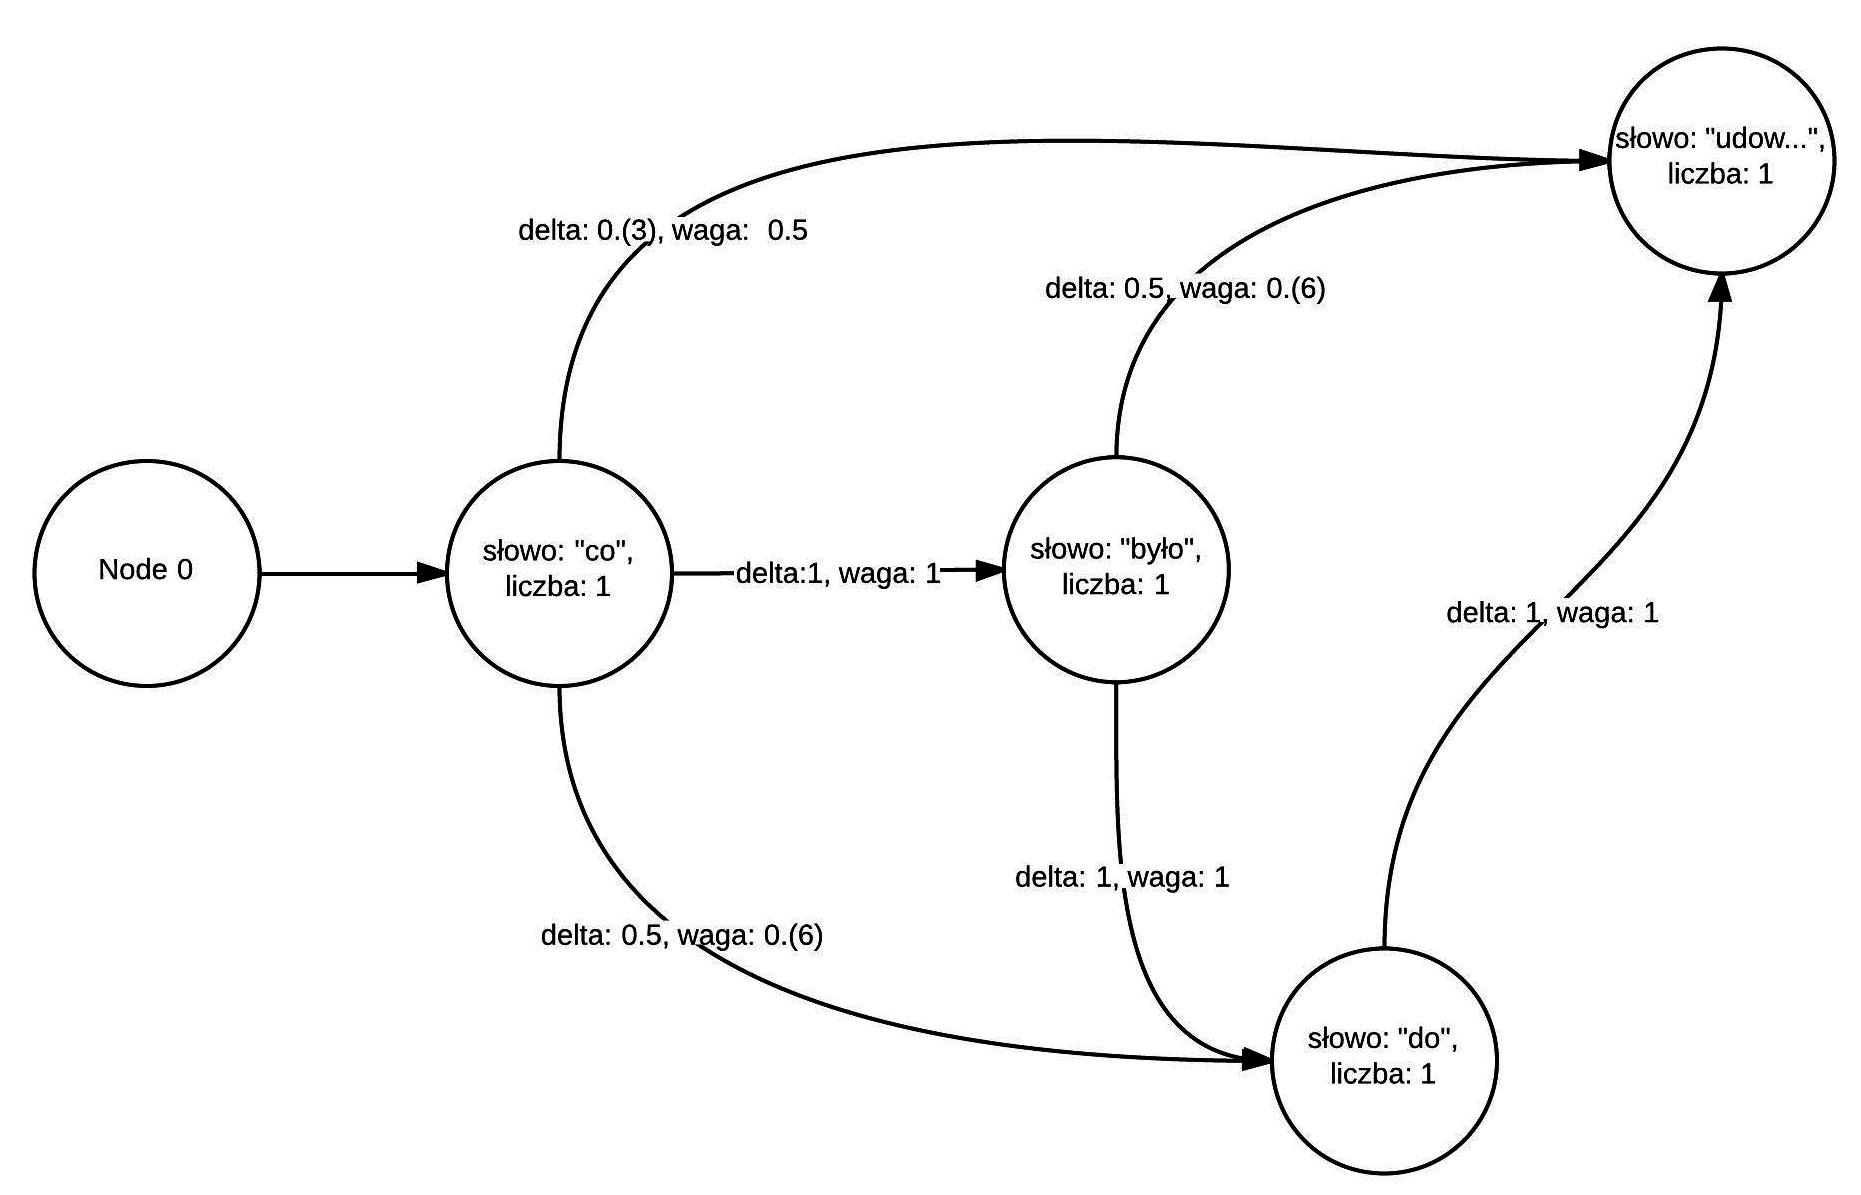
\includegraphics[width=\textwidth]{logic_graph}
    \caption{Przykład reprezentacji sekwencji uczącej w bazie grafowej.}
\end{figure}

Na rysunku \ref{graph:logic_graph} przedstawiona jest logiczna struktura grafu, widziana przez komponenty 5. - 7. Jest to struktura AGDS, powstała na podstawie sekwencji uczącej
$S = \{co, byl{}o, do, udow...\}$. Widoczny jest również domyślny węzeł zerowy(Node 0), obecny w każdej strukturze Neo4j.

